\appendix   % This command is used only once!
%\addcontentsline{toc}{chapter}{APPENDICES}             %toc entry  or:
%\addtocontents{toc}{\parindent0pt\vskip12pt APPENDICES} %toc entry, no page #

\section{Mesh Visualization}

Paraview is program created by Kitware, Inc. which can visualize meshes
and fields on meshes.
It is the program of choice for viewing meshes created by the PUMI libraries.
PUMI API provides a function \emph{pumi$\_$mesh$\_$write} and if this is executed with mesh type ``vtk" for a mesh distributed over two processes:

\begin{verbatim}
  pumi_mesh_write(mesh, "output", "vtk");
\end{verbatim}\vspace{-.5cm}\hspace{1cm}

It would create the files \texttt{output0.vtu}, \texttt{output1.vtu},
and \texttt{output.pvtu}.
Opening the \texttt{output.pvtu} file in Paraview will show users the
mesh.

By default, Paraview will just render the mesh in ``Surface" mode.
Changing this to ``Surface with Edges" will outline each visible element,
actually making the decomposition visible.

Also, the mesh by default is rendered in one ``Solid Color".
There should be other options corresponding to the fields and numberings
that were on this mesh at the time of file writing.
There is usually an ``apf\_part" alternative for files written by APF, which
allows users to see the parallel partitioning of the mesh in color.

When vertices are numbered, it may be useful to display their numbers.
See Section \ref{sec:meshmisc} for information on creating numberings.
Right above the mesh viewing area there is a button to select nodes,
you may also press the ``D" key.

\begin{center}
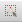
\includegraphics[width=0.05\textwidth]{fig/select_nodes.png}
\end{center}

Click and drag to select all the nodes you want to display.
Then go to \texttt{View->Selection Display Inspector} in the menu and click on
the Point Labels options.
There you can choose what to display.
If you used \texttt{numbering} properly, there should be an option
with the same name that you gave to the numbering.
Note that in some later versions of Paraview, there is a bug which
displays all values as floating point numbers by default.
If you are trying to show \texttt{numbering} values, you may
see strange scientific notation instead.
Click the following icon in the Selection Display Inspector:

\begin{center}

\includegraphics[width=0.05\textwidth]{fig/gear.png}
\end{center}

There you will find a format string option, which you can change
to ``\texttt{\%d}" in order to show integers.

